\begin{titlepage}
\begin{center}
\newcommand{\quickcharcount}[1]{%
  \immediate\write18{texcount -1 -sum -merge -char -q #1.tex output.bbl > #1-chars.sum }%
  \input{#1-chars.sum}%
}
\vspace{1cm}
% \begin{figure}
%         \centering
%         
\includegraphics[width=0.45\textwidth]{Images/itu_logo.png} % højre
% \end{figure}

\begin{figure}
        \centering
        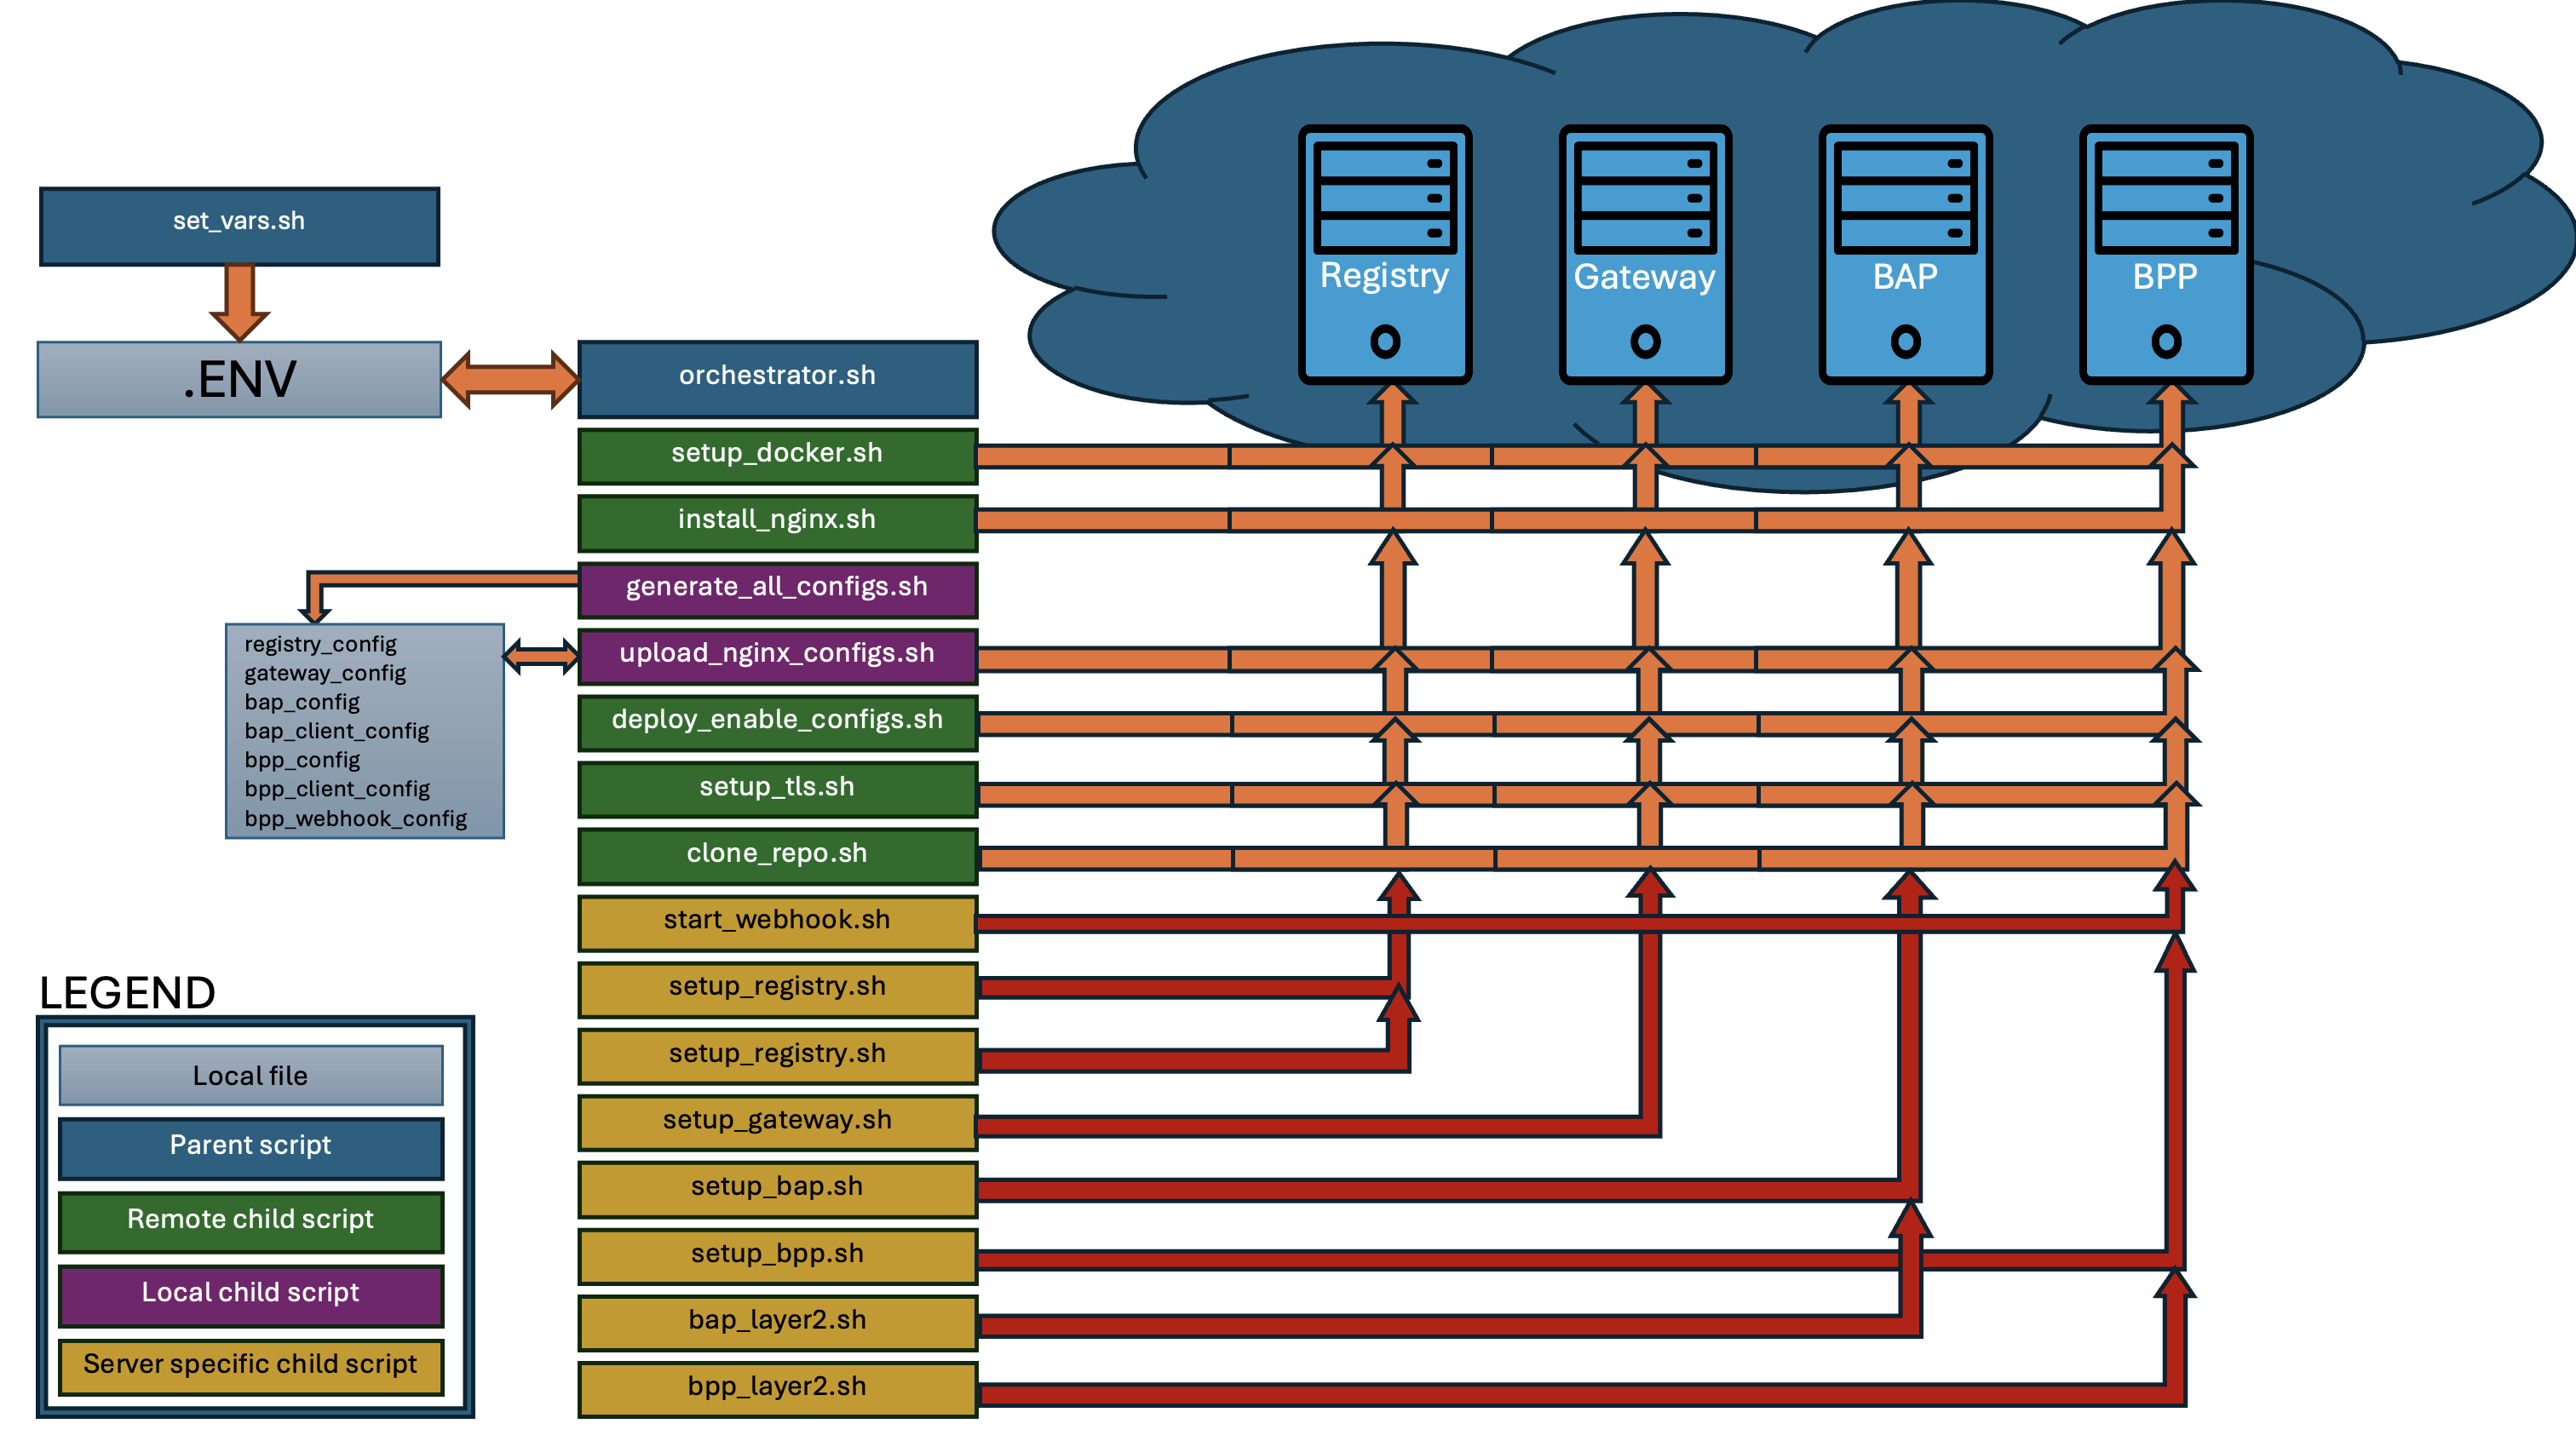
\includegraphics[width=0.85\textwidth]{Images/orchestrator_architecture.png} % højre
\end{figure}

\vspace{1cm}

% Title
{\Large Bachelor Project}\\[0.7em]
\vspace{.5cm}
\hrule
\vspace{.5cm}
{\LARGE \bfseries Decentralizing Digital Markets:}\\[0.5em]
{\Large \titleDocument}
\vspace{.5cm}

\hrule
\vspace{1cm}

\centering

% add your name here
\begin{center}
\setlength{\tabcolsep}{30pt}
\renewcommand{\arraystretch}{1.2}
\begin{tabular}{ll}
    \Large{Name} & \Large{Email} \\\hline
    Frederik Lund Rosenlund & frlr@itu.dk \\
    Rasmus Lundahl Nielsen & raln@itu.dk \\
\end{tabular}
\end{center}

\vspace{1.5cm}
STADS code: BIBAPRO1PE\\
Software Development, BSc\\
IT-University of Copenhagen\\
May 15th, 2025 % Dato for aflevering

\vspace{.5cm} 

\vspace{.5cm}


\end{center}
\end{titlepage}